%%% Template originaly created by Karol Kozioł (mail@karol-koziol.net) and modified for ShareLaTeX use

\documentclass[a4paper,11pt]{article}

\usepackage[T1]{fontenc}
\usepackage[utf8]{inputenc}
\usepackage{graphicx}
\usepackage{xcolor}

\renewcommand\familydefault{\sfdefault}
\usepackage{tgheros}
\usepackage[defaultmono]{droidmono}

\usepackage{amsmath,amssymb,amsthm,textcomp}
\usepackage{enumerate}
\usepackage{multicol}
\usepackage{tikz}

\usepackage{geometry}
\geometry{total={210mm,297mm},
left=25mm,right=25mm,%
bindingoffset=0mm, top=20mm,bottom=20mm}


\linespread{1.3}

\newcommand{\linia}{\rule{\linewidth}{0.5pt}}

% custom theorems if needed
\newtheoremstyle{mytheor}
    {1ex}{1ex}{\normalfont}{0pt}{\scshape}{.}{1ex}
    {{\thmname{#1 }}{\thmnumber{#2}}{\thmnote{ (#3)}}}

\theoremstyle{mytheor}
\newtheorem{defi}{Definition}

% my own titles
\makeatletter
\renewcommand{\maketitle}{
\begin{center}
\vspace{2ex}
{\huge \textsc{\@title}}
\vspace{1ex}
\\
\linia\\
\@author \hfill \@date
\vspace{4ex}
\end{center}
}
\makeatother
%%%

% custom footers and headers
\usepackage{fancyhdr}
\pagestyle{fancy}
\lhead{}
\chead{}
\rhead{}
\lfoot{Assignment \textnumero{} 1}
\cfoot{}
\rfoot{Page \thepage}
\renewcommand{\headrulewidth}{0pt}
\renewcommand{\footrulewidth}{0pt}
%

% code listing settings
\usepackage{listings}
\lstset{
    language=Python,
    basicstyle=\ttfamily\small,
    aboveskip={1.0\baselineskip},
    belowskip={1.0\baselineskip},
    columns=fixed,
    extendedchars=true,
    breaklines=true,
    tabsize=4,
    prebreak=\raisebox{0ex}[0ex][0ex]{\ensuremath{\hookleftarrow}},
    frame=lines,
    showtabs=false,
    showspaces=false,
    showstringspaces=false,
    keywordstyle=\color[rgb]{0.627,0.126,0.941},
    commentstyle=\color[rgb]{0.133,0.545,0.133},
    stringstyle=\color[rgb]{01,0,0},
    numbers=left,
    numberstyle=\small,
    stepnumber=1,
    numbersep=10pt,
    captionpos=t,
    escapeinside={\%*}{*)}
}

%%%----------%%%----------%%%----------%%%----------%%%

\begin{document}

\title{ACEs Assignment \textnumero{} 1}

\author{Bremen University}

\date{16/04/2018}

\maketitle

\section*{Exercise 1: Graph Coloring}

Encode the 3-coloring problem of the Petersen graph into a SAT instance. Give a DIMAC compatible input file and give a list of the meanings of the SAT problem variables. Then, apply a SAT solver to solve the instance. If it has a solution, give the SAT solver’s output along with its interpretation, i.e., the colored graph.

% code
\begin{lstlisting}[label={list:first},caption=Python code-DIMAC generator.]
#assignment 1.1: Petersen graph 3-coloring problem
#output: DIMACS CNF format
print("p cnf 30 100")
nodes_colors = [[11,12,13,14,15,16,17,18,19,20],
                [21,22,23,24,25,26,27,28,29,30],
                [31,32,33,34,35,36,37,38,39,40]]
counter = 0

#every vertex has at least one color assigned
for i in range(10):
    for j in range(3):
        print(nodes_colors[j][i], end=" ")
    print("0")
    counter += 1
    
#every vertex has at most one color assigned
for j in range(10):
    print((-1)*nodes_colors[0][j], (-1)*nodes_colors[1][j], "0")
    counter += 1
for j in range(10):
    print((-1)*nodes_colors[0][j], (-1)*nodes_colors[2][j], "0")
    counter += 1
for j in range(10):
    print((-1)*nodes_colors[1][j], (-1)*nodes_colors[2][j], "0")
    counter += 1

#not have the same color assigned to two nodes that are connected by an edge
#inner part
for j in range(3):
    for i in range(5):
        print((-1)*nodes_colors[j][i], (-1)*nodes_colors[j][(i+2)%5], "0")
        print((-1)*nodes_colors[j][i], (-1)*nodes_colors[j][(i+3)%5], "0")
        print((-1)*nodes_colors[j][i], (-1)*nodes_colors[j][i+5], "0")
        counter += 3
#external part
for j in range(3):
    for i in range(5, 9):
        print((-1)*nodes_colors[j][i], (-1)*nodes_colors[j][i+1], "0")
        counter += 1
    print((-1)*nodes_colors[j][9], (-1)*nodes_colors[j][5], "0")
    counter += 1
\end{lstlisting}

The generated DIMACS compatible code is in "assignment 1-1 DIMACS.txt". The result is:\\
\\
SATISFIABLE\\
v -1 -2 -3 -4 -5 -6 -7 -8 -9 -10 11 -12 -13 -14 15 -16 17 -18 19 -20 -21 -22 -23 24 -25 -26 -27 28 -29 30 -31 32 33 -34 -35 36 -37 -38 -39 -40 0\\

\begin{figure}[h]
\caption{Petersen graph 3-coloring problem}
\centering
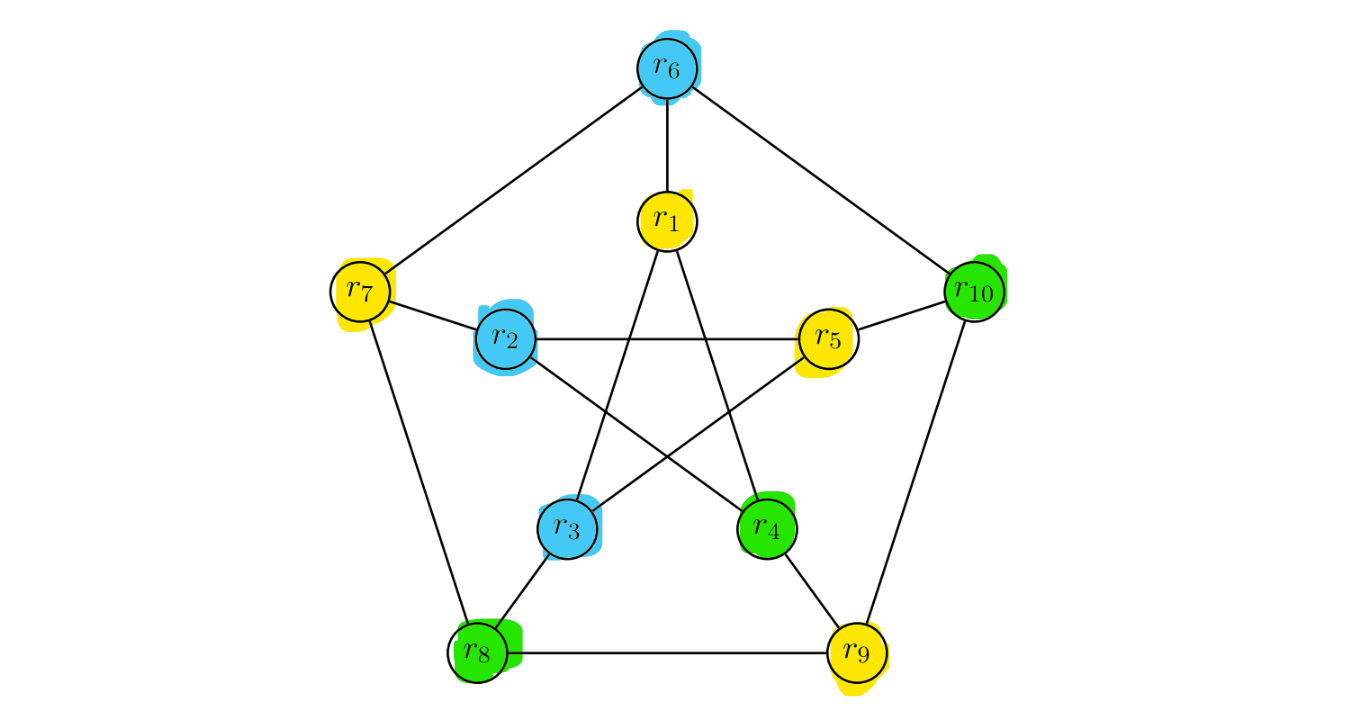
\includegraphics[width=0.8\textwidth]{assignment1.png}
\end{figure}

\section*{Problem 2: Edge coloring}

Describe in a similar style as in the lecture how we can encode the c-edge coloring problem of a graph G = (V, E) into a SAT instance.\\
Every egde has at least one color assigned, as shown in SAT instance.
\begin{equation}
\bigwedge\limits_{e\in E} \bigvee\limits_{c\in \{1,...n\}} x_{e,c}
\end{equation}

Every edge has at most one color assigned.
\begin{equation}
\bigwedge\limits_{c,c'\in \{1,...n\}, c'\neq c} \bigwedge\limits_{e\in E} (\neg x_{e,c} \vee \neg x_{e,c'})
\end{equation}

No two edges that have a joint vertex may have the same color.
\begin{equation}
\bigwedge\limits_{e,e'\in V} \bigwedge\limits_{c \in \{1,...n\}} (\neg x_{e,c} \vee \neg x_{e',c})
\end{equation}

\begin{lstlisting}[label={list:second},caption=Python code-DIMAC generator.]
#assignment 1.1: Petersen graph 3-coloring problem
#output: DIMACS CNF format
print("p cnf 45 165")
edges_colors = [[11,12,13,14,15,16,17,18,19,20,21,22,23,24,25],
                [31,32,33,34,35,36,37,38,39,40,41,42,43,44,45],
                [51,52,53,54,55,56,57,58,59,60,61,62,63,64,65]]
counter = 0

#every edge has at least one color assigned
for i in range(15):
    for j in range(3):
        print(edges_colors[j][i], end=" ")
    print("0")
    counter += 1
    
#every edge has at most one color assigned
for j in range(15):
    print((-1)*edges_colors[0][j], (-1)*edges_colors[1][j], "0")
    counter += 1
for j in range(15):
    print((-1)*edges_colors[0][j], (-1)*edges_colors[2][j], "0")
    counter += 1
for j in range(15):
    print((-1)*edges_colors[1][j], (-1)*edges_colors[2][j], "0")
    counter += 1

#No two edges that have a joint vertex may have the same color.
#inner part
for j in range(3):
#inner - middle
    for i in range(5):
        print((-1)*edges_colors[j][i], (-1)*edges_colors[j][i+5], "0")
        counter += 1
    for i in range(3):
        print((-1)*edges_colors[j][i], (-1)*edges_colors[j][i+7], "0")
        counter += 1
    print((-1)*edges_colors[j][3], (-1)*edges_colors[j][5], "0")
    print((-1)*edges_colors[j][4], (-1)*edges_colors[j][6], "0")
    counter += 2
#inner - inner
    for i in range(5):
        print((-1)*edges_colors[j][i], (-1)*edges_colors[j][(i+2)%5], "0")
        print((-1)*edges_colors[j][i], (-1)*edges_colors[j][(i+3)%5], "0")
        counter += 2
#middle part    
    print((-1)*edges_colors[j][5], (-1)*edges_colors[j][14], "0")
    counter += 1
    for i in range(6,10):
        print((-1)*edges_colors[j][i], (-1)*edges_colors[j][i+5], "0")
        counter += 1
    for i in range(5,10):
        print((-1)*edges_colors[j][i], (-1)*edges_colors[j][i+4], "0")
        counter += 1
#external part        
    for i in range(4):
        print((-1)*edges_colors[j][i+10], (-1)*edges_colors[j][i+11], "0")
        counter += 1
    print((-1)*edges_colors[j][10], (-1)*edges_colors[j][14], "0")
    counter += 1
print(counter)
\end{lstlisting}
The generated DIMACS compatible code is in "assignment 1-2 DIMACS.txt". The result is:\\
UNSATISFIABLE\\
UNSAT\\

\end{document}
